\documentclass{standalone}
\usepackage{tikz}
\usepackage{amsmath}
\usetikzlibrary{matrix,chains,positioning,decorations.pathreplacing,arrows}
\usetikzlibrary{positioning, calc, chains}
\usetikzlibrary{decorations.pathreplacing}
\begin{document}


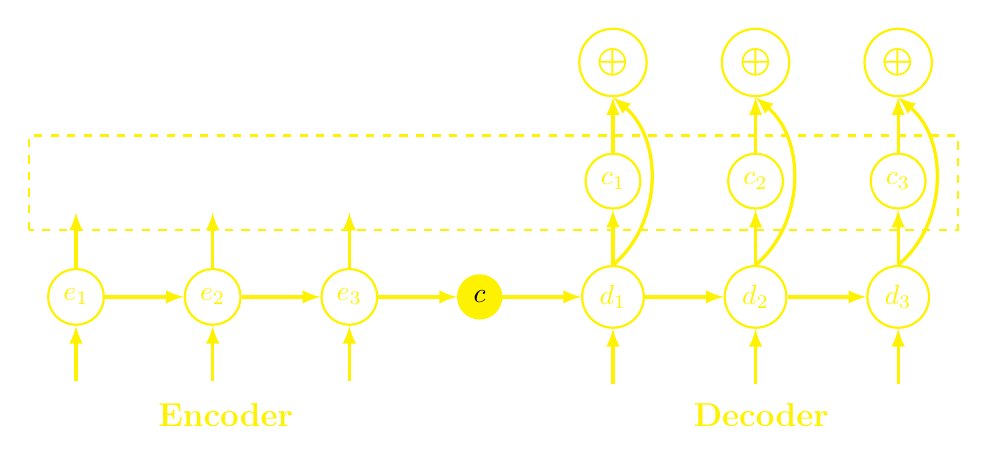
\begin{tikzpicture}[draw=yellow, item/.style={circle,draw,thick,align=center},
itemc/.style={item,on chain,join}]

%encoder
\begin{scope}[start chain=going right,nodes=itemc,every
join/.style={-latex,very thick},local bounding box=chain, xshift=-7cm]
\path 
	node[color=yellow] (e1) {$e_1$} 
	node[color=yellow] (e2) {$e_2$} 
	node[color=yellow] (e3) {$e_3$} 
	node[color=yellow, fill=yellow] (c)  {\textcolor{black}{$c$}} 
	node[color=yellow] (d1) {$d_1$} 
	node[color=yellow] (d2) {$d_2$} 
	node[color=yellow] (d3) {$d_3$}; 
\end{scope}

\foreach \T in {1,2,3} 
{   %encoder
	\draw[very thick,-latex] (e\T.north) -- ++ (0,2em)
	node[above, color=yellow]  {};
	\draw[very thick,latex-] (e\T.south) -- ++ (0,-2em)
	node[below, color=yellow] {};
	
	%decoder
	\draw[very thick,-latex] (d\T.north) -- ++ (0,2em)
	node[above,item, color=yellow] (c\T) {$c_\T$};
	\draw[very thick,latex-] (d\T.south) -- ++ (0,-2em)
	node[below, color=yellow] {};
	
	% hidden states
	\draw[very thick,-latex] (c\T.north) -- ++ (0,2em)
	node[above, item, color=yellow] (h\T) {$\bigoplus$};
	 
	% concat 
   	\path[very thick,-latex] (d\T.north) edge[bend right=50] (h\T.south);   
}

\draw[thick, dashed, draw=yellow] (-7.6, .85) rectangle ++(11.8,1.2);


% captions
\node at (-5.1,-1.5) {\textcolor{yellow}{\large \textbf{Encoder}}};
\node at (1.7,-1.5) {\textcolor{yellow}{\large \textbf{Decoder}}};
\end{tikzpicture}



\end{document}